\documentclass[12pt]{article}
\usepackage{natbib}
\usepackage[french]{babel}
\usepackage[T1]{fontenc}
\usepackage{url}
\usepackage[utf8x]{inputenc}
\usepackage{amsmath}
\usepackage{mathtools}
\usepackage{graphicx}
\graphicspath{{images/}}
\usepackage{parskip}
\usepackage{vmargin}
\usepackage{amssymb}

\title{Modèle de Percolation}								% Title
\date{\today}											% Date

\makeatletter
\let\thetitle\@title
\let\theauthor\@author
\let\thedate\@date
\makeatother

\begin{document}
%%%%%%%%%%%%%%%%%%%%%%%%%%%%%%%%%%%%%%%%%%%%%%%%%%%%%%%%%%%%%%%%%%%%%%%%%%%%%%%%%%%%%%%%%

\begin{titlepage}
	\centering
    
\includegraphics[scale = 0.7]{University.png}\\[1.0 cm]	% University Logo
    \textsc{\LARGE \newline\newline Faculté des Sciences appliquées}\\	% University Name
	\textsc{\Large  INFO0902-1 : Structures de données et algorithmes}\\[0.5 cm]				% Course Code
	\rule{\linewidth}{0.2 mm} \\[0.4 cm]
	{ \huge \bfseries \thetitle}\\
	\rule{\linewidth}{0.2 mm} \\[2 cm]
	
	\begin{minipage}{0.5\textwidth}
		\begin{flushleft} \large
			\emph{Professeur:}\\
			GEURTS Pierre\\
			\end{flushleft}
			\end{minipage}~
			\begin{minipage}{0.4\textwidth}
            
			\begin{flushright} \large
			\emph{Groupe:} \\
			LAMBERMONT Romain\\
            LOUIS Arthur\\
		\end{flushright}
        
	\end{minipage}\\[5 cm]
	
	
    \thedate
    
    
    
	
\end{titlepage}

%%%%%%%%%%%%%%%%%%%%%%%%%%%%%%%%%%%%%%%%%%%%%%%%%%%%%%%%%%%%%%%%%%%%%%%%%%%%%%%%%%%%%%%%%
\thispagestyle{empty}
\tableofcontents
\pagebreak
\setcounter{page}{1}
\section{Analyse Théorique}
\subsection{Description \texttt{UnionFindTree.c}}

\subsection{Complexités \texttt{ufUnion} et \texttt{ufFind}}

\subsection{Structure \texttt{Percolation.c}}

\subsection{Complexité en temps et espace de \texttt{thresholdEstimate} par listes}

\subsection{Complexité en temps et espace de \texttt{thresholdEstimate} par arbres}
\newpage
\section{Analyse Empirique}
\subsection{Centilles et seuil critique de percolation}
\begin{figure}[!h]
    \centering
    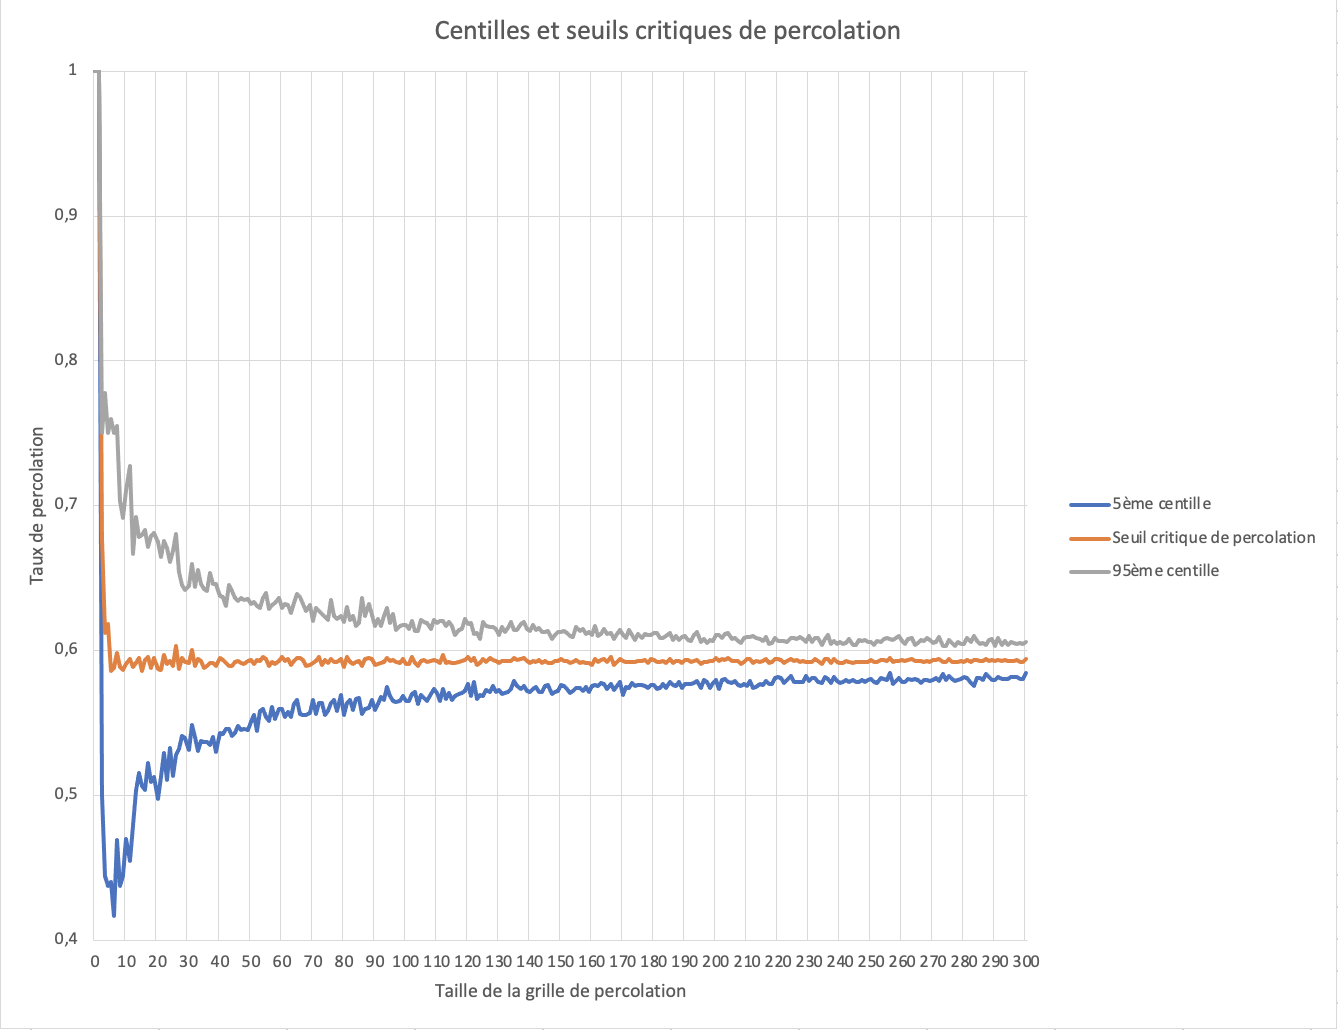
\includegraphics[scale = 0.4]{Centilles.png}
    \caption{Graphique des centilles et seuils critiques de percolation en fonction de la taille de la grille}
    \label{fig:centilles_taux}
\end{figure}

\subsection{Temps d'exécution en fonction de l'implémentation}

\begin{figure}[!h]
    \centering
    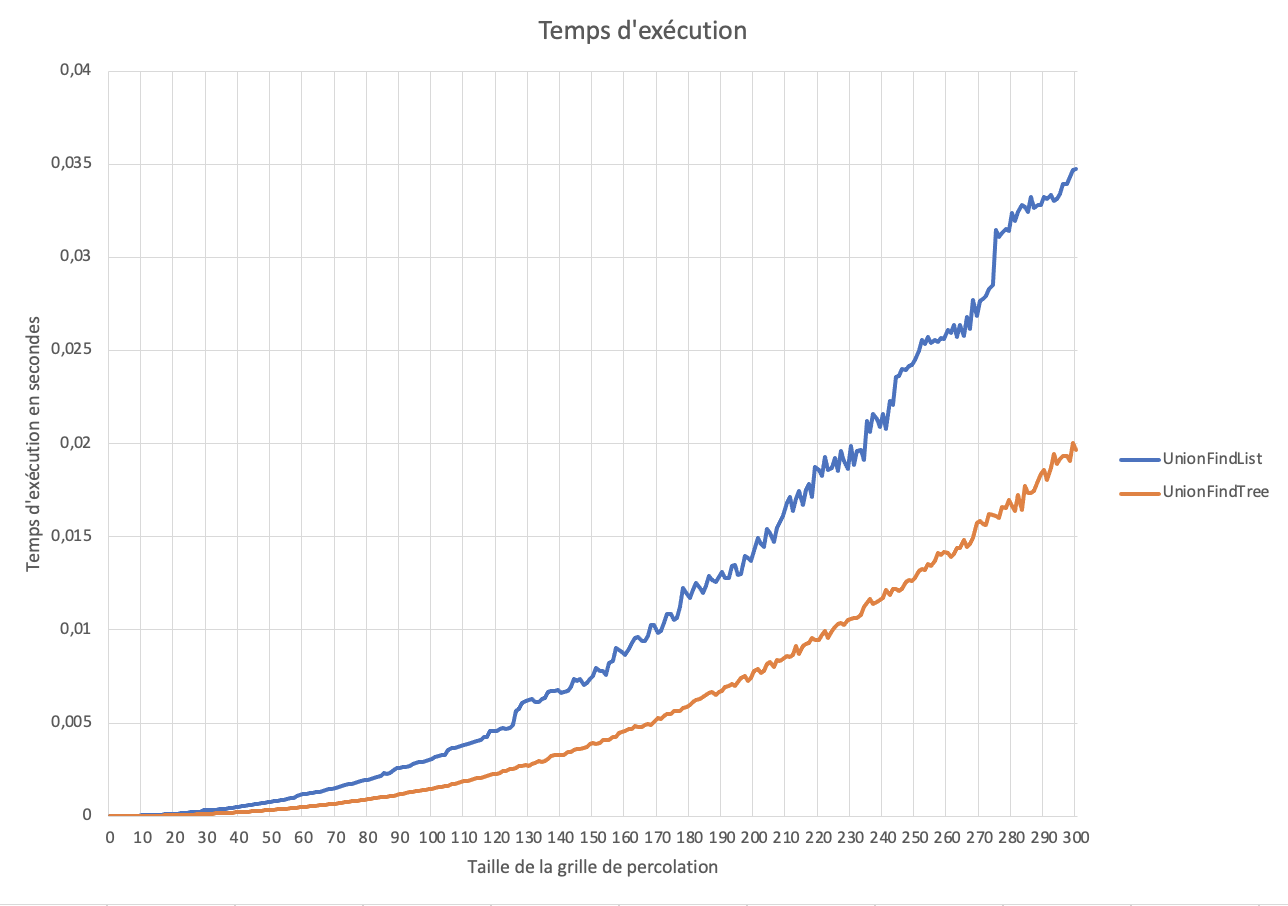
\includegraphics[scale = 0.4]{Temps.png}
    \caption{Graphique des temps d'exécution en fonction de la méthode d'implémentation et de la taille de la grille}
    \label{fig:my_label}
\end{figure}
\subsection{Discussion des courbes}
\end{document} 